
\section{Evaluation}\label{sec:evaluation}

In this section, we experimentally analyze various real-time aspects
of the DeepPicar. This includes
(1) measurement based worst-case execution time (WCET) analysis of
deep learning inferencing,
(2) the effect of using multiple cores in accelerating inferencing,
(3) the effect of co-scheduling multiple deep neural network models,
and 
(4) the effect of co-scheduling memory bandwidth intensive co-runners.

\subsection{Setup}

The Raspberry Pi 3 Model B platform used in DeepPicar equips a Boardcom
BCM2837 SoC, which has a quad-core 64bit ARM Cortex-A53 cluster,
running at up to 1.2GHz. Each core has 16K private I\&D caches, and all
cores share a 512KB L2 cache.
The chip also includes Broadcom's Videocore IV
GPU, although we did not use the GPU in our evaluation due to the lack
of sofware support (Tensorflow is not compatible with the GPU).
For software, we use Ubuntu MATE 16.04, Tensorflow 1.1 and python
2.7. We disabled DVFS (dynamic voltage frequency scaling) and
configure the clock speed of each core at the maximum 1.2GHz.

\subsection{Inference Timing for Real-Time Control}

For real-time control of a car (or any robots), the control loop
frequency must be sufficiently high so that the car can quickly
react to the changing environment and its internal states. In general,
control performance improves when the frequency is higher, though
computation time and the type of particular physical system are
factors in determining a proper control loop latency. While a standard
control system may be comprized of multiple control loops with
differning control frequencies---e.g., a inner control loop for lower-level
PD control, a outer loop for motion planning, etc.---DeepPicar's
control loop is a single layer, as shown earlier in
Figure~\ref{fig:controlloop}, as a single deep neural network
replaces the traditional multi-layer control pipline. (Recall
Figure~\ref{fig:end-to-end-control} on the differences between the
standard robotics control vs. end-to-end deep learning approach).
This means that the DNN interference operation must be completed
within the inner-most control loop update frequency. To understand
achievable control-loop update frequencies, we experimentally measured
the execution times of DeepPicar's DNN inference operations.

% 50-200Hz for quadcopters:
% https://robotics.stackexchange.com/questions/231/what-frequency-does-my-quadcopter-output-sense-calculate-output-update-loop-need 
% https://quadmeup.com/pid-looptime-why-it-is-not-only-about-frequency/

\begin{figure}[t]
  \centering
  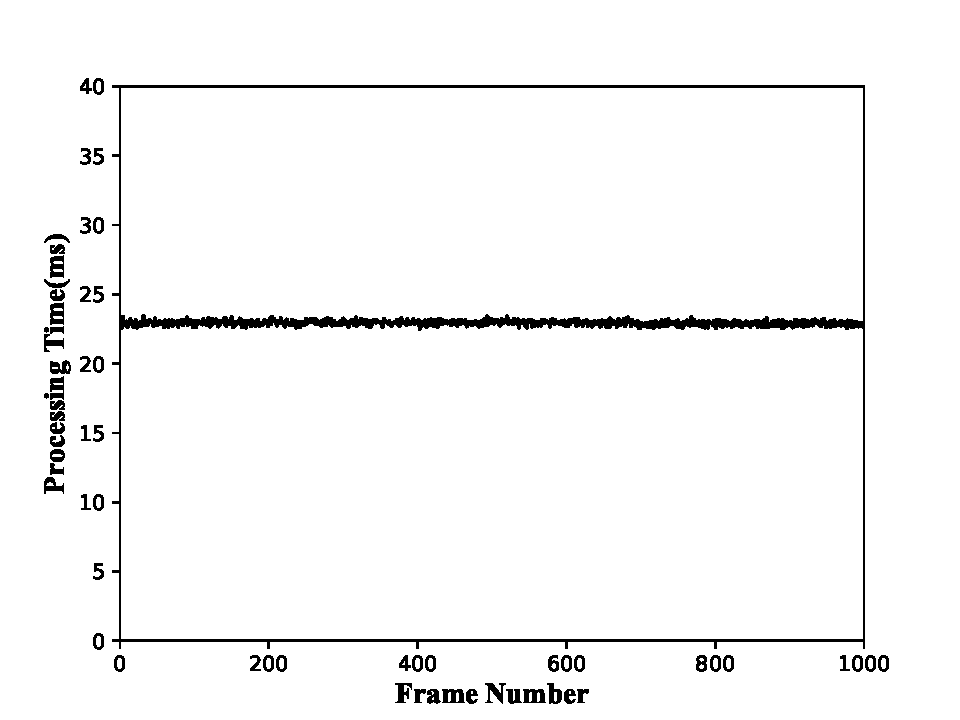
\includegraphics[width=.5\textwidth]{figs/Fig7_new}
  \caption{DeepPicar's control loop processing times over 1000 input image frames.}
  \label{fig:control-loop-timing}
\end{figure}

\begin{table}[t]
  \centering
  \begin{tabular} {| c | r | r | r | r |}
    \hline
    \textbf{Operation} & \textbf{Mean} & \textbf{Max} &   \textbf{99pct.} & \textbf{Stdev.} \\ \hline
    Image capture        & 2.28  &  4.94 &  4.54  & 0.52 \\ \hline
    Image pre-processing & 3.09  &  4.60 &  3.31  & 0.10 \\ \hline
    DNN inferencing      & 37.30 & 51.03 & 45.48  & 2.75 \\ \hline
    Total Time           & 42.67 & 56.37 & 50.70  & 2.80 \\ \hline
  \end{tabular}
  \caption{Control loop timing breakdown.}
  \label{tbl:control-loop-breakdown}
\end{table}

Figure~\ref{fig:control-loop-timing} shows the measured control loop 
processing times of the DeepPicar over 1000 image frames (one per each
control loop). We omit the first frame processing time for cache
warmup. Table~\ref{tbl:control-loop-breakdown} shows the time
breakdown of each control loop. Note that all four CPU cores of the
Raspberry Pi 3 were used by the Tensorflow library when performing the
DNN inference operations.

First, as expected, we find that the inference operation
dominates the control loop execution time, accounting about 85\% of
the execution time.
Second, more importantly, we also find that the measured average
execution time of a single control loop is 42.67 ms, or 23.4 Hz and
the 99 percentail time is 50.70ms.
This means that the DeepPicar can operates
at about 20 Hz control frequency in real-time using only the on-board
Raspberry Pi 3 computing platform, without needing any remote computing
resources. We consider these results respectable given the complexity
of the deep neural network  and the fact that the inference operation
performed by Tensorflow only utilizes the CPU cores of the
Raspberry Pi 3 (its GPU is not supported by Tensorflow.)

In comparison, NVIDIA's DAVE-2 system, which has the exact same neural
network architecture, is reportedly run at 30 Hz~\cite{Bojarski2016},
just a bit faster than the DeepPicar. Although we believe it was not
limited by their computing platform (we will experimentally compare
performance differences among multiple embedded computing platforms,
including NVIDIA's Jetson TK2, later in
Section~\ref{sec:comparison}), the fact that the low-cost
Raspberry Pi 3 can achieve similar real-time control performance is
surprising.

\subsection{Effect of the Core Count to Inference Timing}

In this experiment, we investigate the scalability of performing
inference operation of DeepPicar's nueral network with respect to the
number of cores. As noted earlier, the Raspberry Pi 3 platform has
four Cortex-A53 cores and the Tensorflow 
provides a programmable mechanism to to adjust how many cores to be
used by the library. Leveraging this feature, we repeat the
same experiment described in the previous subsection with varying
number of CPU cores---from one to four.


\begin{figure}[h]
  \centering
  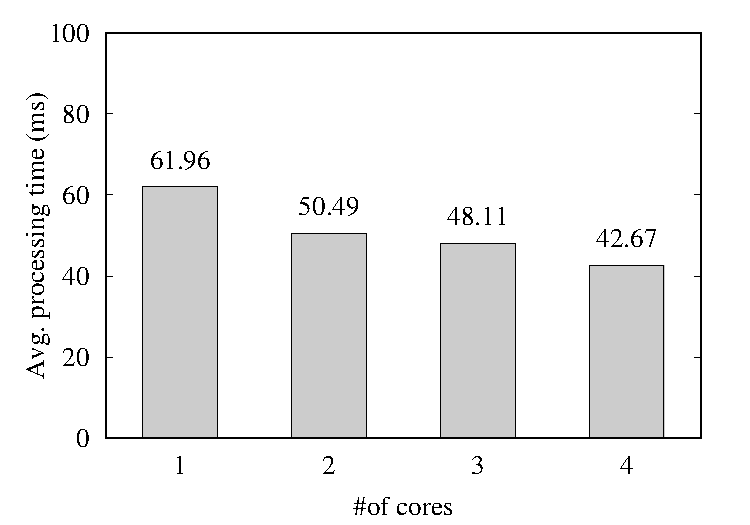
\includegraphics[width=.45\textwidth]{figs/perf_vs_corecnt}
  \caption{Average control loop execution time vs. \#of CPU
    cores.}
  \label{fig:perf-vs-corecnt}
\end{figure}
    %% \fixme{instead of the total control loop time, use the
    %%   average of DNN inferencing time.}}

%% \begin{table}[h]
%%   \centering
%%   \begin{tabular} {| c | l | l | l | l | l | l | l | l | l |}
%%     \hline
%%     \textbf{\#of cores} & \textbf{Mean} & \textbf{Max} & \textbf{99pct} & \textbf{Stdev} \\ \hline 
%%     1 & 61.96 & 66.00 & 63.31 & 0.51\\ \hline
%%     2 & 50.49 & 71.55 & 70.03 & 3.16 \\ \hline
%%     3 & 48.11 & 72.22 & 58.45 & 4.18 \\ \hline
%%     4 & 42.67 & 56.37 & 50.70 & 2.80 \\
%%     \hline
%%   \end{tabular}
%%   \caption{Execution time statistics vs. \#of CPU cores.}
%% \end{table}

Figure~\ref{fig:perf-vs-corecnt} shows the average execution times of
the control loop as we vary the number of cores used by the
Tensorflow. As expected as we assign more cores, the average execution
time decreases---from 61.96 ms on a single core to 42.67 ms on four
cores (a 30\% improvement). However, the improvement is far from ideal
linear scaling. In particular, from 2 cores to 3 cores, the
improvement is mere 2.38ms (or 4\%). In short, we find that the
scalability of DeepPicar's deep neural network is not ideal on the
platform. We do not know whether it is due to the limitations of
Tensorflow's multicore implementation or it's the model's inherent
characteristics. 

The poor scalability opens up the possibility of consolidating
multiple different tasks or different nueral network models rather
than allocating all cores for a single nueral network model. For
example, it is conceivable to use four cameras and four different
neural network models, each of which is trained seperately and
executed on a single dedicated core. Assuming we use the same network
architecture for all models, then one might exepct to achieve up to
15 Hz using one core (given 1 core can deliver 62ms average
execution time). In the next experiment, we investigate the
feasibility of such a scenario.

%% It may not always be the case that all four cores of the Raspberry Pi
%% 3's Cortex A-53 CPU can be used solely for the purpose of operating an
%% autonomous vehicle. Thus, we test how the number of cores utilized for
%% real-time operations affects the DeepPicar's overall ability to
%% function as an autonomous vehicle platform.

%% The performance of the DeepPicar is summarized in Table III. The
%% DeepPicar performed better, on average, when it utilized more
%% cores. With 4 cores, it was able to meet the vast majority of its
%% deadlines, doing so in almost 99\% of the input frames. The platform
%% performed the worst when using only 1 core, as it was unable to meet
%% any of its deadlines.  On average, using 3 cores instead of 2 only had
%% a performance increase of approximately 2 ms, so the addition of one
%% core in that specific case offers  relatively little improvement. One
%% important observation is that the performance was more consistent when
%% only 1 core was used. As a result, the use of multiple cores is very
%% beneficial in terms of reducing the time it takes to complete
%% inference operations, but may result in times that are more volatile.

\subsection{Effect of Co-scheduling Multiple DNN Models}

In this experiment, we launch multiple instances of DeepPicar's DNN
model at the same time and measure its impact to their inference
timings. In particular, we are interested in how shared resource
contention affect inference timing.

%% We also test the capability of the DeepPicar to run multiple models at
%% the same time, and whether each model can successfully perform within
%% the given deadline. Specifically, the platform is tested in the cases
%% of running 2 and 4 models simultaneously. For each case, all models
%% are allocated an equal number of cores. That is, 2 models are given 2
%% cores each and 4 models are given 1 core each.

\begin{figure}[h]
  \centering
  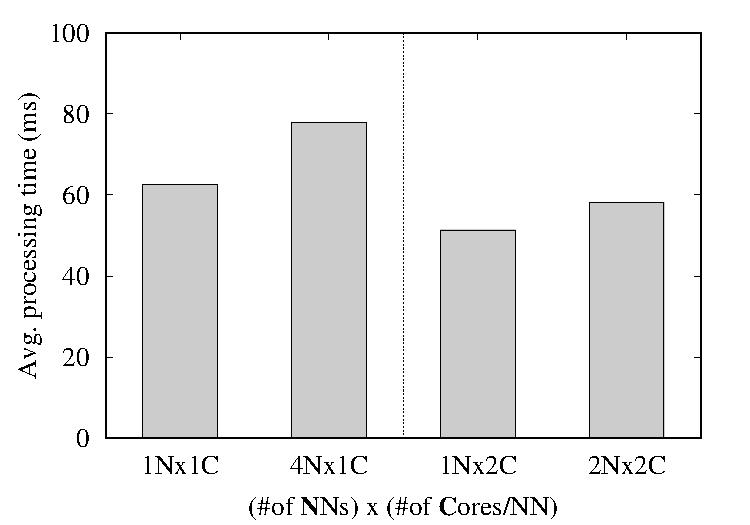
\includegraphics[width=.45\textwidth]{figs/perf_vs_modelcnt}
  \caption{Timing impact of co-scheduling multiple DNNs. 1x1: one DNN
    model using one CPU core; 4x1: four DNN models each using one CPU;
    1x2: one DNN model using two CPU cores; 2x2: two DNN models each
    using two CPU cores.} 
  \label{fig:perf-vs-modelcnt}
\end{figure}

%% \begin{figure}[h]
%%   \centering
%%   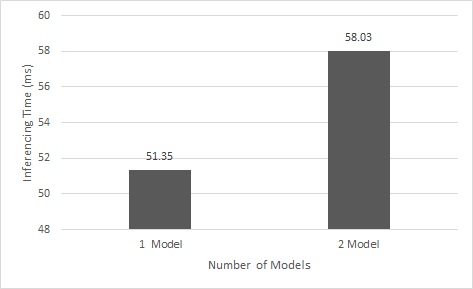
\includegraphics[width=.5\textwidth]{figs/2ModelChart}
%%   \caption{ Change in inferencing time when 2 models are run concurrently. }
%% \end{figure}
%% \begin{figure}[h]
%%   \centering
%%   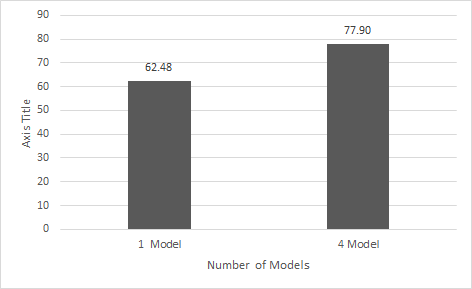
\includegraphics[width=.5\textwidth]{figs/4ModelChart}
%%   \caption{Change in inferencing time when 4 models are run simultaneously. }
%% \end{figure}


Figure~\ref{fig:perf-vs-modelcnt} shows the results. In the figure,
X-axis shows the system configuration: \#of DNN models x \#of CPU
cores\/DNN. For example, '4x1' means running four DNN models each of
which is assigned to run on one CPU core, whereas '2x2' means running
two DNN models, each of which is assigned to run on two CPU
cores. The Y-axis shows the average inference timing.
Two bars in the left show the impact of co-scheduling four DNN
models. Compared to executing a single DNN model on one CPU core
(1x1), when four DNN models are co-scheduled (4x1), each model
suffers an average inference time increase of approximately 15 ms,
$\sim$24\%. On the other hand, when two DNN models, each using two CPU
cores, are co-scheduled, the average inference timing is increased by
about 7 ms, or 10\%, comapred to the baseline of running one model
using two CPU cores. 

%% The results for the 2 model test are outlined in Figure 3 and Table
%% IV, and the 4 model test is summarized in  Figure 4 Table V. In the
%% the 2 model test, both of the models showed average inference time
%% increases of around  5-7 ms, $\sim$10\%, when compared to a baseline
%% of 1 model running on two cores.

%% \begin{table}[h]
%% \centering
%%   \begin{tabular} {| l | l | l |}
%%   \hline
%%   \textbf{num models} & 1 & 2 \\ \hline
%%   \textbf{L1 refs} &  3.04E+10 &  3.04E+10 \\ \hline
%%   \textbf{L1 misses} & 4.78E+08 & 4.91E+08 \\ \hline
%%   \textbf{L1 miss \%} & 1.58 & 1.61 \\ \hline
%%   \textbf{L2 refs} & 3.31E+09 &  3.91E+09 \\ \hline
%%   \textbf{L2 misses} & 3.68E+08 & 4.62E+08 \\ \hline
%%   \textbf{L2 miss \%} & 11.12 & 10.88 \\ \hline
%%   \end{tabular}
%%   \caption{ Effect of 2 simulatneous models on cache accesses. }
%% \end{table}

%% \begin{table}[h]
%% \centering
%%   \begin{tabular} {| l | l | l |}
%%   \hline
%%   \textbf{num models} & 1 & 4 \\  \hline
%%   \textbf{L1 refs} & 2.78E+10 & 2.79E+10 \\ \hline
%%   \textbf{L1 misses} & 4.36E+08 & 4.53E+08 \\ \hline
%%   \textbf{L1 miss \%} & 1.57 & 1.63 \\ \hline
%%   \textbf{L2 refs} & 2.83E+09 & 3.36E+09 \\ \hline 
%%   \textbf{L2 misses} & 3.59E+08 & 4.43E+08 \\ \hline
%%   \textbf{L2 miss \%} & 12.68 & 13.19 \\ 
%% \hline
%%   \end{tabular}
%%   \caption{ Effect of 4 concurrent models on cache accesses. }
%% \end{table}

\begin{figure}[h]
  \centering
  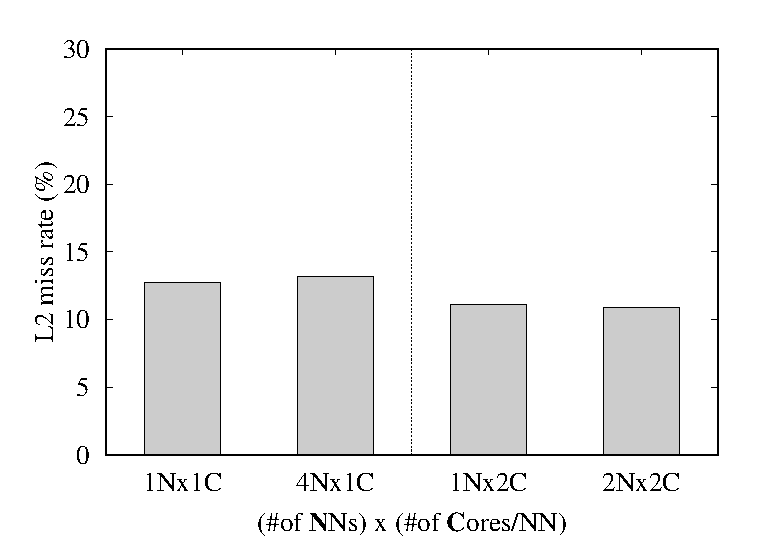
\includegraphics[width=.45\textwidth]{figs/l2missrate_vs_modelcnt}
  \caption{L2 cache miss rates of different neural network and core
    assignments. X-axis is the same as Figure~\ref{fig:perf-vs-modelcnt}.} 
  \label{fig:l2missrate-vs-modelcnt}
\end{figure}

These increases in inference times in the co-scheduled scenarios are
expected and likely caused by contention in the shared hardware
resources such as the shared L2 cache and/or the DRAM controller.
To further analyze the source of contention, we use hardwawre
performance counters of the processor. Specifically, we measure L2
miss rates of the DNN models first in isolation and then after
co-scheduling another models. If the shared L2 cache is the primary
source of inteference, then the measured L2 miss rates would
increase. Figure~\ref{fig:l2missrate-vs-modelcnt} shows the results.
As can be see in the figure, L2 miss rates are largely unchanged
regardless whether multiple models are co-scheduled or not. This
suggests that the shared L2 cache is not the bottleneck that caused
execution time increases. In other words, DNN models appear to be not
sensitive to the shared L2 cache space. % L2 partitioning is probably
                                % not going to be useful.
Instead, we hypothesize that it is likely caused by the memory
controller---the only other major shared hardware source---where
memory requests from different CPU cores contend, which would result
in increased memory access latency. While some Intel processors
provide uncore hardware counters that can measure average memory
access latency~\cite{ye2016maracas}, we were not able to identify
whether such hardware counters exist in the BCM2837 processor of
Raspberry Pi 3 due to the lack of documentation. Instead, in the next
experiment, we use memory intensive synthetic benchmarks to test the
hypothesis.

%% The increase in inference times, however, was not the result of
%% increased cache misses due to additional accesses. For all models, the
%% number of L1 misses was always $\sim$1.6\% of all  references. In the
%% 2 model test, L2 cache misses remained at $\sim$11\% of all
%% references, and each model in the 4 model test missed $\sim$13\% of
%% all L2 references. 

%% In all multimodel tests, it was found that a greater number of models
%% run simultaneously resulted in interference that led to a noticable
%% increase in the average inferencing time that wasn't attributable to a
%% change in cache misses. Instead, the overall time increases can most
%% likely be traced to an increase in cache latency. Even if the models
%% had a consistent number of cache hits, it is highly probable that the
%% contention for the cache increased the access time for each model,
%% consequently increasing the time it took for the models to execute
%% their operations.

%% In terms of real-time performance under a WCET of 50
%% ms, the DeepPicar was unsatisfactory in all multimodel tests. On
%% average, the 2 model test saw models miss their deadline by 6-8 ms,
%% and the 4 model test was worse as each model went over their deadlines
%% by 27-29 ms. As a result, it can be ascertained that, if a WCET of 50
%% ms is required, DeepPicar would not be able to perform as necessary.

\subsection{Effect of Co-scheduling Memory Performance Hogs}

In order to determine how contended DRAM requests affect the DNN
inference timing of the DeepPicar, we use a synthetic memory
intensive benchmark from the IsolBench suite~\cite{Valsan2016}.

We run a single DNN model one core, and
co-schedule an increasing number of the memory intensive synthetic
benchmarks~\footnote{We use the \emph{Bandwidth} benchmark in the
  IsolBench suite, with the following command line parameters: \texttt{\$
  bandwdith -a write -m 16384}}, on the remaining idle cores.

\begin{figure}[h]
  \centering
  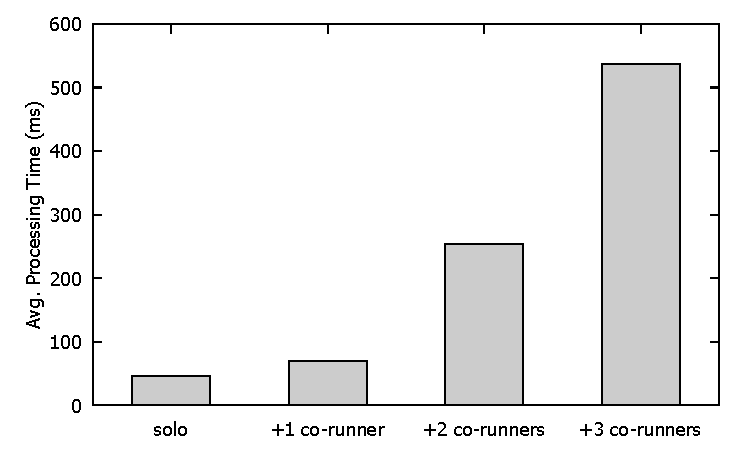
\includegraphics[width=.45\textwidth]{figs/perf_vs_bandwidth}
  \caption{Effect of memory performance hogs on the DNN
    inferencing. The DNN model uses Core 0 and memory-hog co-runnes
    use the rest of the cores.}
  \label{fig:}
\end{figure}

%% \begin{table}[h]
%% \centering
%%   \begin{tabular} {| l | l | l | l | l | l |}
%%   \hline
%%   \textbf{num cores} & 1 & 2 & 3 \\ \hline
%%   \textbf{L1 refs} & 3.16E+10 & 3.17E+10 & 3.06E+10 \\ \hline
%%   \textbf{L1 misses} & 5.41E+08 & 5.35E+08 & 4.98E+08 \\ \hline
%%   \textbf{L1 miss \%} & 1.71 & 1.69 & 1.62 \\ \hline
%%   \textbf{L2 refs} & 3.49E+09 & 3.23E+09 & 3.21E+09 \\ \hline
%%   \textbf{L2 misses} & 8.05E+08 & 7.54E+08 & 4.98E+08 \\ \hline
%%   \textbf{L2 miss \%} & 23.05 & 23.37 & 15.51 \\ 
%%   \hline
%%   \end{tabular}
%%   \caption{ Effect of benchmarks on cache accesses. }
%% \end{table}

Figure~\ref{fig:} shows the normalized execution time and L2 miss-rate
of the DNN model running on the Core 0 as a function of the number of
co-scheduled memory intensive synthetic benchmarks. First, as we
increase the number of co-runners, the DNN model's execution times are
increased---by up to 9.6X---even though the DNN model is running on a
dedicated core (Core0). On the other hand, the DNN model's L2
cache-miss rates are not increase as much. This suggests that
the DNN model's exeuction increase cannot be fully explained by
increased L2 cache-misses. Instead, as we hypothesized in the previous
experiment, the increased memory pressure from the co-scheduled memory
intensive benchmarks is the primary cause of the DNN model's execution
time increase. Therefore, we conclude that DeepPicar's DNN model is
more senstive to DRAM access latency than L2 cache space.

This observation suggests that shared cache partitioning
techniques~\cite{Gracioli2015,Kim2016} may not be effective isolation
solutions for DeepPicar as its AI workload is more sensitive to memory
performance. Instead, memory controller focused isolation solutions,
either hardware or software-based ones (e.g.,~\cite{Guo2017,Yun2013}),
may be more important. Although our observation is made on a single
hardware platform running on a single DNN workload, we suspect that
many AI workloads may exhibit similar characteristics.

%% The presence of the benchmark(s) had a noticable effect on the
%% DeepPicar, with all tests showing increases in inferencing
%% operations. The least change happened when the model was run on 3
%% cores, and a single benchmark was run on the final core. Even with a
%% slight increase in the number of L2 cache misses, inferencing was able
%% to be completed in under 100 ms. The other tests, however, showed
%% dramatic changes when the model was run on 1 and 2 cores. In both
%% instances, L2 misses rose to $\sim$23\% of all references. The
%% additional benchmark in the 1 core test was even more detrimental as
%% the average inferencing time was at least 150 ms longer than when the
%% model used 2 cores.  

%% With the introduction of synthetic benchmarks, the DeepPicar failed to
%% comply with the 50 ms WCET across all tests run. Even in the best
%% case, inferencing operations take twice as long as the deadline to
%% complete. As a result, if benchmarks were required to run during
%% autonomous operation, the DeepPicar wouldn't be capable of meeting its
%% deadlines.

\begin{table*}[h]
  \centering
  \begin{tabular}{|c|c|c|c|}
    \hline
    Item    & Raspberry Pi 3 (B)   & Intel UP                  & NVIDIA Jetson TX2\\
    \hline
            & BCM2837              & X5-Z8350 (Cherry Trail)   & Tegra TX2 \\
    CPU     & 4x Cortex-A53@1.2GHz/512KB L2  &
              4x Atom@1.92GHz/2MB L2 &
              4x Cortex-A57@2GHz/2MB L2 \\
            &              &              & 2x Denver@2.0GHz/2MB L2 (not used)  \\
    \hline
    GPU     &  VideoCore IV (not used)    &
               Intel HD 400 Graphics (not used) &
               Pascal 256 CUDA cores   \\
    \hline
    Memory  & 1GB LPDDR2   &  2GB DDR3L     & 8GB LPDDR4              \\
    \hline
  \end{tabular}
  \caption{Compared embedded computing platforms}
  \label{tbl:platforms}
\end{table*}

\subsection{Summary of the Findings}
So far, we have evaluated DeepPicar's real-time
characteristics from the perspective of end-to-end deep learning based
real-time control, and made several observations.

First, we find that DeepPicar's computing platform,
the Raspberry Pi 3 Model B, offers adquate computing capacity to
perform real-time control of the RC car at 20 Hz frequency (or
50ms per control loop). Given the complexity of the DNN we use, we
were pleasantly suprised by this finding. The time breakdown shows that
the DNN inferencing operation, perforemd by the Tensorflow library,
dominates the execution time, which is expected.

Second, we find that scalability of Tensorflow's DNN inference 
implementation is limited: We find that using all four cores are 
only about 30\% better than using just a single core.

Third, we find that consolidating multiple DNN models---on different CPU
cores---is feasible as we find: (1) DNN performance using a single
core is not much worse than using multiple cores; (2) multiple DNN
models running simultaneously do not cause severe interference with
each other.

Lastly, we however find that consolidating memory (DRAM) performance
intensive applications could jeopadize DNN performance because DNN
performance appear very sensitive to memory performance; we observe up
to 9.6X slowdown in DNN performance by co-scheduling synthetic memory 
bandwidth intensive applications on idle cores.

%% is capable of successfully completing all
%% necessary inferencing operations within a given deadline of 50
%% ms. Between these operations, it was discovered that the angle
%% prediction time of the model was the dominating step in the processing
%% time of a single frame. The other operations were found to execute in
%% very little time, with either one taking 5 ms at most

%% When running a
%% single model, DeepPicar performed the best when it used all 4 cpu
%% cores, as it was able to process a frame in 43 ms on average. This
%% feat can still be accomplished when running a single model on 3 cpu
%% cores, and is also possible when using 2 cores. The only time in which
%% the Pi can't run a single model under 50 ms is when only 1 core is
%% used. This was also the case when multiple models were run
%% concurrently as no models were able to consistently complete inference
%% operations in under 50 ms.

%% However, the DeepPicar was shown to be capable of handling other
%% potential WCETs. If given a larger deadline, the capabilities of
%% DeepPicar as an autonomous vehicle platform would be greatly
%% increased. For example, if tested with a deadline of 66.67 ms, or 15
%% fps, the platform would have passed several of the experiments
%% performed. In actuality, the DeepPicar would have only been
%% unsatisfactory in the 4 model test where it would have missed the
%% deadlines by $\sim$10 ms, and the benchmark tests, where  
%% it would still miss by $\sim$33 ms at best.


%% In our platform, three main real-time tasks are performed during autonomous operation. In order, these 
%% operations are: (1) capturing and reading the input frame from the designated camera or video stream, 
%% (2) preprocessing the acquired frame so that it is compatible with the DNN, and (3) feeding the frame 
%% to, and getting the angle prediction from, the model. We aim to determine which operation(s), if any, 
%% require the most time to be performed.

%% In order to determine which operation(s) take the longest to execute, we measured the time it 
%% took for each step to be completed. For this experiment, all four of the Pi's cpu cores were utilized, 
%% and only one model was run. As is shown in Table II, the angle prediction operation consumes the 
%% majority of the processing for each frame. Furthermore, the time it takes for the operation to 
%% complete is volatile, and can range anywhere between 30 ms and 50 ms for any particular frame. On the 
%% other hand, both the frame capture and preprocessing operations take substantially less time 
%% and are relatively more consistent in their times, at 2 ms and 3 ms, respectively. 


%% In evaluating the real-time efficacy of the DeepPicar, the methodology is consistent across all 
%% experiments. The performance of the platform is measured over a set of 1001 video frames that are 
%% each individually fed to the model. The processing time for the first frame is omitted as, due to 
%% cache warmup, it is uncharacteristically high and doesn't
%% accurately represent the Picar's capabilities.  
%% A WCET of 50 ms, or 20 Hz, is used as a baseline to assess the platform's ability to complete all 
%% necessary real-time operations in a timely manner.

%% We seek to determine if the DeepPicar is capable of consistently executing all necessary functions 
%% before their given deadlines. In the case of our platform, it has to process every given frame and get 
%% the predicted angles from the model within a WCET of 50 ms. In order to determine if this was achievable, 
%% we tested the platform by running a single model that utilized all 4 cpu cores and measured the time it 
%% took for each frame to be processed. The performance of the DeepPicar can be seen in Figure 6. We found 
%% that DeepPicar was able to completely process the vast majority of the provided frames within 50 ms, and 
%% was unable to do so for very few frames.

%% In our platform, three main real-time tasks are performed during autonomous operation. In order, these 
%% operations are: (1) capturing and reading the input frame from the designated camera or video stream, 
%% (2) preprocessing the acquired frame so that it is compatible with the DNN, and (3) feeding the frame 
%% to, and getting the angle prediction from, the model. We aim to determine which operation(s), if any, 
%% require the most time to be performed.

%% In order to determine which operation(s) take the longest to execute, we measured the time it 
%% took for each step to be completed. For this experiment, all four of the Pi's cpu cores were utilized, 
%% and only one model was run. As is shown in Table II, the angle prediction operation consumes the 
%% majority of the processing for each frame. Furthermore, the time it takes for the operation to 
%% complete is volatile, and can range anywhere between 30 ms and 50 ms for any particular frame. On the 
%% other hand, both the frame capture and preprocessing operations take substantially less time 
%% and are relatively more consistent in their times, at 2 ms and 3 ms, respectively. 
